\begin{example}
Προσδιορίστε το μετασχηματισμό $A_v$ που ευθυγραμμίζει δοσμένο διάνυσμα $\vec{v}$ με το μοναδιαίο διάνυσμα $\vec{k}$ κατά μήκος του θετικού μέρους του άξονα των $z$.

\end{example}

\begin{solution}
	Τα ακόλουθα βήματα απαιτούνται για το ζητούμενο μετασχηματισμό. 
	
\textbf{Βήμα 1:} Περιστροφή του διανύσματος $v$ γύρω από τον άξονα $x$ κατά γωνία $\theta_1$ έτσι ώστε το $v$ να πέφτει στο πάνω μέρος του επιπέδου $xz$ (διάνυσμα $v_1$, Σχήμα \ref{fig:10}

\begin{center}
	Βασικός πίνακας μετασχηματισμού $R_{\theta_1, x}$.
\end{center}

\textbf{Βήμα 2:} Περιστροφή του διανύσματος $v_1$ γύρω από τον άξονα των $y$ κατά γωνία $-\theta_2$ έτσι ώστε ώστε το $v_1$ να πέσει πάνω στο θετικό μέρος του άξονα των $z$ (διάνυσμα $v_2$ Σχήμα \ref{fig:11}).

\begin{center}
	Βασικός πίνακας μετασχηματισμού $R_{-\theta_2, x}$.
\end{center}


\begin{figure}[h!]
	\begin{center}
		\begin{minipage}[b]{0.48\textwidth} % Top-left image
		%    \centering
		    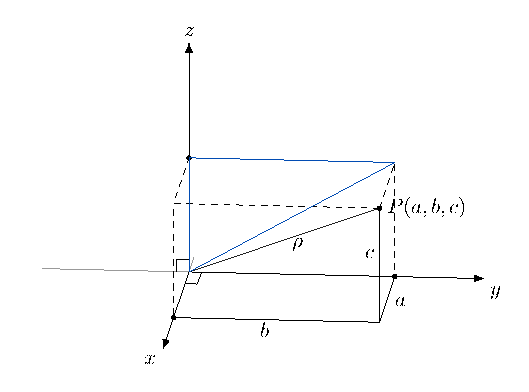
\includegraphics[scale=1]{Chapter3/Av1.pdf}
%		    \captionof{figure}{}
		\end{minipage}%
	\hfill
		\begin{minipage}[b]{0.48\textwidth} % Top-right image
		%    \centering
		    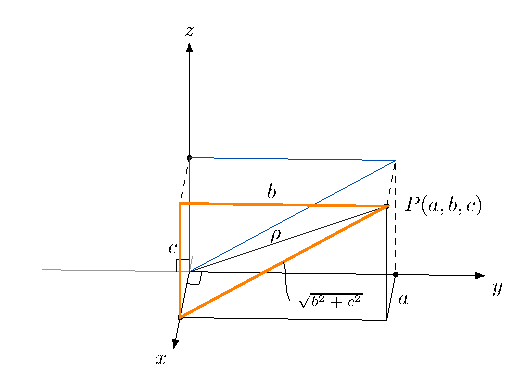
\includegraphics[scale=1]{Chapter3/Av2.pdf}
%		    \captionof{figure}{Βήμα 4}
		\end{minipage}
	\end{center}
	\caption{Διάνυσμα $v$ που καλούμαστε να ευθυγραμμίσουμε με το μοναδιαίο διάνυμα $\vec{k}$ του άξονα $z$}
\end{figure}


\begin{figure}[h!]
	\begin{center}
		\begin{minipage}[b]{0.48\textwidth} % Top-left image
		%    \centering
		    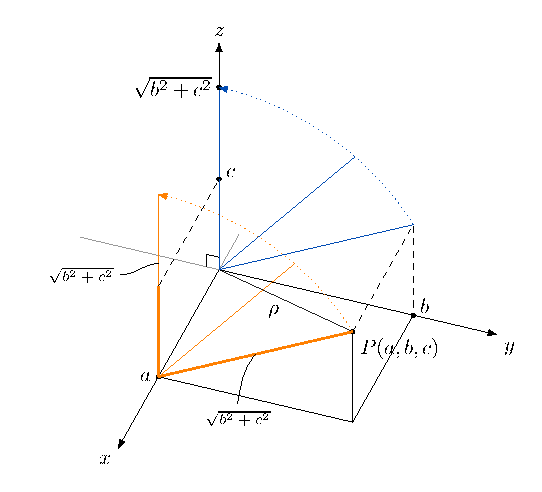
\includegraphics[scale=1]{Chapter3/Av3.pdf}
%		    \captionof{figure}{}
		\end{minipage}%
	\hfill
		\begin{minipage}[b]{0.48\textwidth} % Top-right image
		%    \centering
		    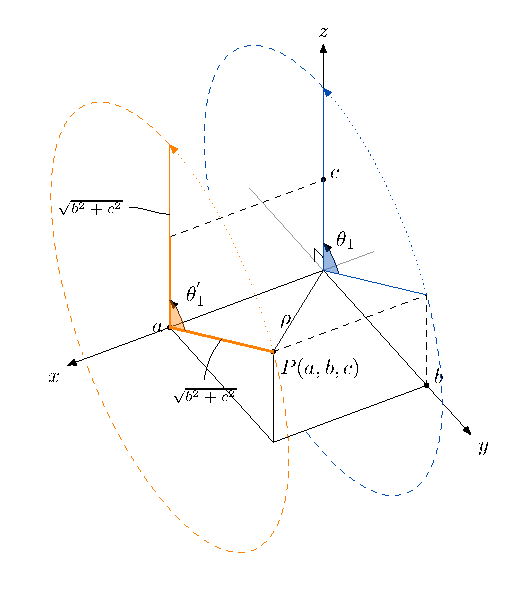
\includegraphics[scale=1]{Chapter3/Av4.pdf}
%		    \captionof{figure}{Βήμα 4}
		\end{minipage}
	\end{center}
	\caption{Βήμα 1: Περιστροφή του διανύσματος $v$ γύρω από τον άξονα $x$ κατά γωνία $\theta_1$ έτσι ώστε το $v$ να πέσει στο επίπεδο $xz$}
\end{figure}


\begin{figure}[h!]
	\begin{center}
%		\begin{minipage}[b]{0.48\textwidth} % Top-left image
		%    \centering
		    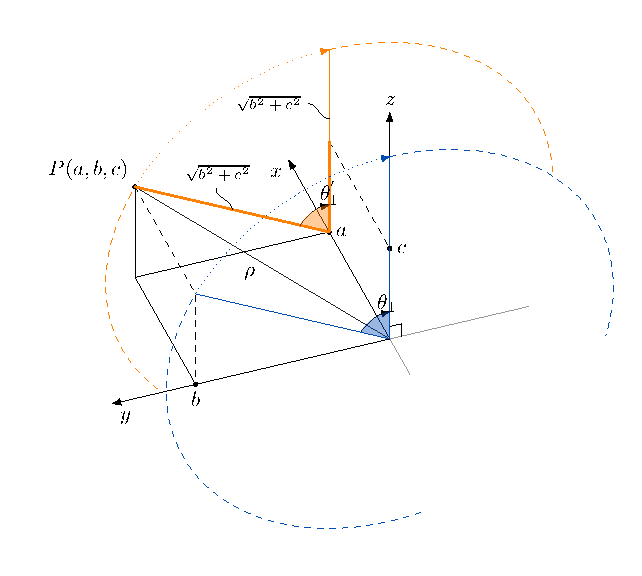
\includegraphics[scale=0.8]{Chapter3/Av4-reverse.pdf}
%		    \captionof{figure}{}
%		\end{minipage}%
	\end{center}
	\caption{Διαφορετική όψη στροφής διανύσματος $v$ γύρω από τον άξονα $x$}		
\end{figure}


\begin{figure}[h!]
	\begin{center}
		\begin{minipage}[b]{0.48\textwidth} % Top-left image
		%    \centering
		    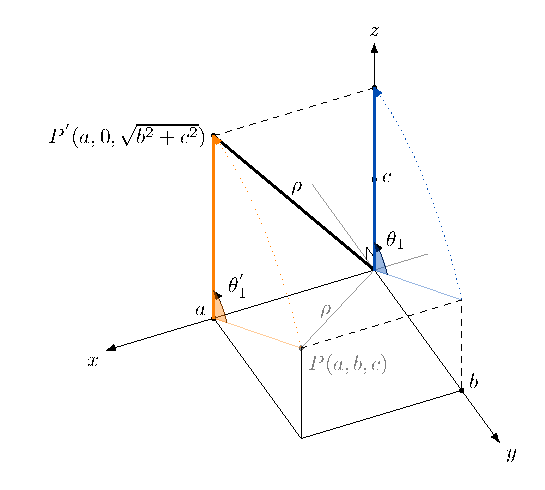
\includegraphics[scale=1]{Chapter3/Av5.pdf}
%		    \captionof{figure}{}
		\end{minipage}%
	\hfill
		\begin{minipage}[b]{0.48\textwidth} % Top-right image
		%    \centering
		    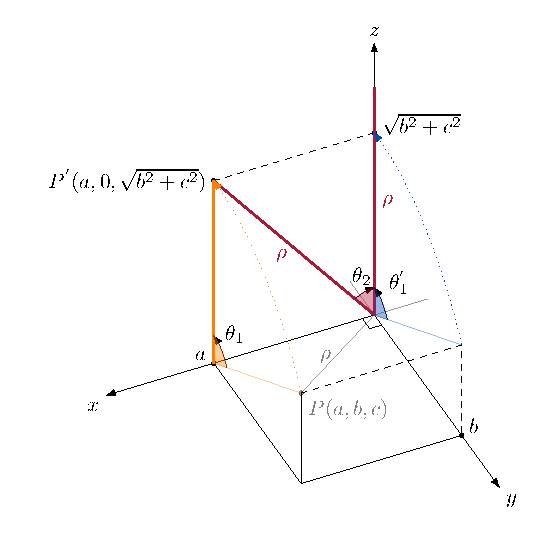
\includegraphics[scale=1]{Chapter3/Av6.pdf}
%		    \captionof{figure}{Βήμα 4}
		\end{minipage}
	\end{center}
	\caption{Βήμα 2: Περιστροφή του διανύσματος $v_1$ γύρω από τον άξονα των $y$ κατά γωνία $-\theta_2$ έτσι ώστε ώστε το $v_1$ να πέσει πάνω στο θετικό μέρος του άξονα των $z$}
\end{figure}

Ο ζητούμενος πίνακας θα προκύψει σαν σύνθεση των παραπάνω βασικών μετασχηματισμών αφού όμως πρώτα προσδιοριστούν οι γωνίες $\theta_1$ και $\theta_2$.

\underline{Προσδιορισμός των γωνιών $\theta_1$ και $\theta_2$:} Από το Σχήμα  \ref{fig:11} παρατηρούμε ότι η ζητούμενη γωνία $\theta_1$ θα προσδιοριστεί από τη γωνία που σχηματίζει η προβολή του $v$ στο επίπεδο $yz$ με τον άξονα των $z$. (υποθέτουμε ότι $b$ και $c$ δεν είναι και τα δύο μηδέν). Από το τρίγωνο $OP'B$ \textcolor{red}{check} προκύπτει:

\begin{align*}
	\sin{\theta_1} &= \cfrac{b}{\sqrt{b^2 + c^2}} \\
	\cos{\theta_1} &= \cfrac{c}{\sqrt{b^2 + c^2}}
\end{align*}


Ο πίνακας περιστροφής \(R_{\theta_1, x}\) ισούται με:

\[
R_{\theta_1, x} =
\begin{bmatrix}
1 & 0 & 0 & 0\\
0 & \cfrac{c}{\sqrt{b^2 + c^2}} & \cfrac{-b}{\sqrt{b^2 + c^2}} & 0\\
0 & \cfrac{b}{\sqrt{b^2 + c^2}} & \cfrac{c}{\sqrt{b^2 + c^2}} & 0 \\
0 & 0 & 0 & 1
\end{bmatrix}
\]

Επιδρώντας με αυτόν τον πίνακα στο διάνυσμα $v(a, b, c)$ προκύπτουν οι συντεταγμένες του $v_1(x, y, z)$:

\[
		\begin{bmatrix}
			x \\
			y \\
			z \\
			1
		\end{bmatrix}
	=
		R_{\theta_1, x} \cdot 
		\begin{bmatrix}
			a \\
			b \\
			c \\ 
			1
		\end{bmatrix}
	= 
		\begin{bmatrix}
			1 & 0 & 0 & 0\\
			0 & \cfrac{c}{\sqrt{b^2 + c^2}} & \cfrac{-b}{\sqrt{b^2 + c^2}} & 0\\
			0 & \cfrac{b}{\sqrt{b^2 + c^2}} & \cfrac{c}{\sqrt{b^2 + c^2}} & 0 \\
			0 & 0 & 0 & 1
		\end{bmatrix}
	\cdot 
		\begin{bmatrix}
			a \\
			b \\
			c \\ 
			1
		\end{bmatrix}
	=
		\begin{bmatrix}
			a \\
			0 \\
			\sqrt{b^2+c^2} \\ 
			1
		\end{bmatrix}
\]

Για τον προσδιορισμό της γωνίας $\theta_2$ από το τρίγωνο $OQQ'$ (Σχήμα \ref{fig:11}) προκύπτει:

\begin{align*}
	\sin{(-\theta_2)} &= = -\sin{\theta_2} -\cfrac{a}{\sqrt{a^2 + b^2 + c^2}} \\	
	\cos{(-\theta_2)} &= \cos{\theta_2} = \cfrac{\sqrt{b^2 + c^2}}{\sqrt{a^2 + b^2 + c^2}}
\end{align*}

Τελικά, ο ζητούμενος μετασχηματισμός $A_v$ θα ισούται με:

\[
	A_v = R_{-\theta_2, y} \cdot R_{\theta_1, x}
\]

Αντικαθιστώντας τις προηγούμενες γωνίες στους πίνακες $R_{-\theta_2, y}, R_{\theta_1, x}$ και θέτοντας $\lambda = \sqrt{b^2 + c^2}$, προκύπτει:

\[
	A_v =
	\begin{bmatrix}
		\cfrac{\lambda}{|v|} & \cfrac{-ab}{\lambda |v|} & \cfrac{-ac}{\lambda |v|} & 0 \\
		0 & \cfrac{c}{\lambda} & \cfrac{-b}{\lambda} & 0 \\
		\cfrac{a}{|v|} & \cfrac{b}{|v|} & \cfrac{c}{|v|} & 0 \\
		0 & 0 & 0 & 1
	\end{bmatrix}, \ \text{όπου} \ |v| = \sqrt{a^2 + b^2 + c^2}
\]


\begin{remark}
	Εάν \(b\) και \(c\) ισούνται με μηδέν, τότε \(\lambda = 0\). Σε αυτή την περίπτωση απαιτείται μόνο μία περιστροφή \(90^\circ\) ως προς τον άξονα των \(y\). Τότε $v= a\vec{i}$, δηλαδή το δοσμένο διάνυσμα βρίσκεται επί του άξονα $x$. Δηλαδή:

	\[
		A_v = R_{-\theta_2, y} =
		\begin{bmatrix}
			0 & 0 & \cfrac{-a}{|a|} & 0 \\
			0 & 1 & 0 & 0 \\
			\cfrac{a}{|a|} & 0 & 0 & 0 \\
			0 & 0 & 0 & 1
		\end{bmatrix}
	\]
\end{remark}


\begin{remark}	
	Με τον ίδιο τρόπο μπορούμε να υπολογίσουμε τον αντίστροφο μετασχηματισμό \(A_v^{-1}\), που ευθυγραμμίζει το μοναδιαίο διάνυσμα \(\vec{k}\) με το δοσμένο διάνυσμα \(v\). Πιο συγκεκριμένα:
	
	\[
	A_v^{-1} 
		= \left(R_{-\theta_2, y} \cdot R_{\theta_1, x}\right)^{-1} 
		= R_{\theta_1, x}^{-1} \cdot R_{-\theta_2, y}^{-1}
		= R_{-\theta_1, x} \cdot R_{\theta_2, y} 
		= 	\begin{bmatrix}
				\cfrac{\lambda}{|v|} & 0 & \cfrac{a}{|v|} & 0 \\
				\cfrac{-ab}{\lambda |v|} & \cfrac{c}{\lambda} & \cfrac{b}{|v|} & 0 \\
				\cfrac{-ac}{\lambda|v|} & \cfrac{-b}{\lambda} & \cfrac{c}{|v|} & 0 \\
				0 & 0 & 0 & 1
			\end{bmatrix}
	\]
\end{remark}


\begin{remark}	
	Με τη βοήθεια του μετασχηματισμού \(A_v\) μπορούμε να ταυτίσουμε οποιονδήποτε δοσμένο άξονα στον χώρο με κάποιον από τους \(O_x, O_y, O_z\). Έτσι μπορούμε να ανάγουμε το πρόβλημα της στροφής ως προς ένα οποιοδήποτε άξονα \(R\) του χώρου σε πρόβλημα στροφής ως προς τον άξονα \(O_x, O_y\) ή \(O_z\) με τον οποίο θα έχουμε ταυτίσει τον \(R\).  
\end{remark}

	
\end{solution}